\chapter{Anforderungen der Impactanalyse}

    Für eine Umsetzung einer automatischen regulativen Impactanalyse, welche die beschriebenen betrieblichen Prozesse des Anforderungsmanagements und der Nachweisführung berücksichtigt und die Lifecycle und Struktur regulatorischen Anforderungen / Anforderungsdokumenten darstellen kann, bedarf es einigen Voraussetzungen.  
    Nach der Marktanalyse der \ac{EGRC} Plattformen durch Gartner\cite{app_gartner} unterstützt Compliance Management ,,Compliance Fachpersonal bei der Dokumentation, bei Workflows, Berichterstattung und der Visualisierung von Control Objectives [...]``\cite[S.4 (übersetzt)]{app_gartner} für verschiedene branchenspezifischen Regularien, Vereinbarungen und Anforderung externe oder interne Anforderungen.       
    Die Impactanalyse oder dessen mögliche Implementation in Rahmen einer Anwendung, einer \ac{EGRC} Plattform oder eines Businessprozesses sollte folglich in der Lage sein, einen Mehrwert im Sinne einer Automatisierung oder einer Verringerung des händischen Workloads darzulegen.

    % Genauer sollte eine Implementation im Rahmen dieser Arbeit -- mittels einer Impactanalyse -- herausarbeiten, welche Teile einer Complianceangabe zu einer ATM/ANS-Komponente/-System durch eine Konsolidierung externer Anforderungsdokumente    
    % Die erarbeiteten Anforderungen sollen folglich auch als Kriterien für die Analyse und Bewertung der zwei Datenquellen dienen, um dessen Mehrwert im Sinne dieser Aufgabe zu bestimmen.  

    
% \begin{quote}
% \textcolor{red}{Der Zweck dieses Kapitels soll es sein, vor der Analyse der Datenquellen, Anforderungen herauszuarbeiten, an denen die Quellen bewertet werden können und weiter eine Impact Analyse erstellt werden kann.}
% \end{quote}

\section{Ziel der Impactanalyse}
% \begin{quote}
% \textcolor{green}{Seite füllen (mindestens)}
% \end{quote}

Ziel der \textit{Regulatory Change Impact Analysis (RCIA)} im Rahmen dieser Implementation ist es, eine Liste jener Anforderungen zu erhalten, welche für die Erbringung der Compliance relevant ist und durch die Änderung betroffen ist. 
Eine Complianceangabe gilt folglich als \textit{betroffen}, sowie die durch diese Complianceangabe abgedeckte Anforderung verändert, ersetzt, gelöscht oder durch ein anderes Anforderungsdokument -- oder eine andere Anforderung -- konsolidiert wurde.
Auch neue Anforderungen, hervorgehend aus neuen Anforderungsdokumenten oder der Ergänzung/Konsolidierung bestehender Dokumente, sollten durch die Analyse erkannt und je nach ihrer bewerteten Bedeutung entsprechend berücksichtigt werden.   
Diese Abbildung hilft folglich dabei, den Umfang größerer regulatorischer Änderungen oder Konsolidierungen besser auf einen kleineren -- für das Projekt relevanten -- Rahmen herunterzubrechen und die Effizienz sowie die Qualität der Nachweisführungsprozesse zu optimieren. 
Hersteller der betroffenen Komponenten könnten so, auf Basis dieser Analyse, einfach und übersichtlich betroffene Angaben bzgl. der Compliance ändern und fortan eine hohe Qualität der Nachweisführung sicherstellen.

Neben den Ergebnissen der Impact Analyse und dessen Verwendung in den entsprechenden Nachweisführungsprozessen werden im Zuge der Analyse Datensätze erarbeitet, die auch einen Mehrwert für andere Aufgabenbereiche erwirtschaften kann. 

% Die Automatisierung dieser Analyse bedarf, dass alle Anforderungen in einem Format vorliegen, in dem diese maschinell eingelesen und analysiert werden können. 
% Weiter muss das Format in der Lage sein, inhaltliche wie strukturelle Änderungen der externen Anforderungsdokumente identifizieren oder erarbeiten zu können.  



\pagebreak

    
\section{Modellierung der Daten} 

Die Basis der Analyse bedarf der Existenz eines umfassenden Datensatzes, welcher -- unabhängig von dessen Semantik -- in der Lage ist, regulative Anforderungen, ATM/ANS Komponenten, ATM/ANS Systeme, jeweils mit allen wichtigen zugehörigen Informationen, Metadaten, Lifecycle sowie dessen Beziehungen untereinander abzubilden.
Im Folgenden sollen hierzu Anforderungen erarbeitet und erörtert werden, die eine Analyse unter dem oben definierten Ziel ermöglichen.


\subsection{Regulative Anforderungen}\label{model_anforderungen}


Regulative (externe) Anforderungen beschreiben im Folgenden alle Anforderungen und Definition, welche von gesetzgebenden -- oder hierdurch berechtigten -- Parteien verfasst wurden und eine fortlaufende Bedeutung für die Erklärung der Compliance einer ATM/ANS-Komponente / eines ATM/ANS-Systems hat.   
Im Rahmen dieser Analyse bilden diese Anforderungen den volatilen Teil, aus welchen die zu analysierenden Änderungen hervorgehen.
Dementsprechend bedarf es einer Datendarstellung, welche in der Lage ist, die entsprechenden Lifecycle und Änderungen der Anforderungen inkl. aller wichtigen Informationen integer abzubilden.   
Wichtige Anforderungen an eine solche Abbildung beinhalten:

\subsubsection{Eindeutige Kennung}

    Um eine einheitliche Nachweisführung sicherzustellen, muss durch die Datenmodellierung gewährleistet sein, dass Anforderungen -- auch über Konsolidierungen oder strukturelle Änderungen der Anforderungsdokumente hinweg -- eindeutig identifiziert werden können.
    Sowie die Anforderungsdokumente und dessen Herausgeber keine eindeutige, struktur- und zeitunabhängige Identifizierung der  einzelnen Anforderungen zur Verfügung stellen, bedarf es eines eigenen Prozesses, zur Durchsetzung eigener Kennungsmethoden.  
Die Granularität, mit welcher Textabschnitte identifiziert werden können, gilt es gesondert in Bezug auf die Struktur der einzelnen Anforderungsdokumente herauszuarbeiten.

Im Falle von EU Verordnungen oder anderen Gesetzestexten sind die Kennung eines Textabschnittes zumeist an die Struktur des Dokumentes gebunden. 
In diesem Falle ist die Kennung einer Anforderung in einem Dokumente auch unmittelbar mit dessen Position in der Gliederung verknüpft. 
In diesen Fällen gilt es zu prüfen, ob strukturelle Änderungen der Anforderungsdokumente Auswirkungen, die Nummerierung bestehender Textabschnitte haben kann.
Im Beispiel von digitalen Verordnungen der EU\footnote{Publiziert durch das Amt für Veröffentlichungen der Europäischen Union (FMX Format)} besteht aus Basis der Dokumentation die Möglichkeit, dass die Struktur und Nummerierung Textabschnitte im Rahmen einer Konsolidierung oder Korrektur überarbeitet werden\footnote{Nach der Dokumentation zu Annotationen bzgl. Änderungen (siehe ,,CLG.MDFO/MDFC``) im FMX Format kann die Nummerierung ersetzt werden (siehe Codes \textit{(NN): new numbering}, \textit{(ON): old numbering})\cite[vgl S. 76-79]{eu_fmx4_proc}}. 
Auch wenn derartige Änderungen nicht im Sinne der Integrität des Anforderungsdokumentes getätigt werden und eine eigene Prüfung der -- für ATM/ANS-Equipment relevanten -- Dokumente ergab, dass kein etwaiger Fall in den Dokumenten gefunden wurde, so gilt es im Einzelfall zu eruieren, ob eine strukturelle Identifizierung einzelner Anforderungen eine ausreichend integre Identifizierungsmethode darstellt. 

% sich deshalb sehr wahrscheinlich nur auf Ausnahmesituationen oder sehr kleine Änderungen kleinerer geordneter Listen bezieht, 

\subsubsection{Regulative Quelle}

Die \textit{regulative Quelle} einer Anforderung soll im Folgenden definieren, aus welchem Anforderungsdokument sich eine gewisse Anforderung ableitet. 
Diese Angabe soll folglich sicherstellen, dass auch komplexere Lifecycle von Anforderungen, und dessen Änderungsgesetzen\footnote{Definition hier entsprechend  \textit{amending acts} (engl.) \cite{eu_consolidation}} adäquat abgebildet werden können.
Im möglichen Falle einer Änderung zweiten Grades, bspw. der Korrektur eines Änderungsgesetzes, kann durch den Verweis auf das Änderungsgesetz als \textit{regulative Quelle}, auch dessen Korrektur festgestellt werden. 
Alle konsolidieren Dokumente, jeden Grades, werden somit in den digitalen Lifecycle des Datenmodells mitaufgenommen und entsprechend abgebildet und berücksichtigt.  

Sowie -- durch die Analyse -- erschlossen, bietet dieses Attribut Auskunft über die Versionierung individueller Anforderungen und ermöglicht es, einfach nachzuvollziehen, welche Anforderungen durch welche Konsolidierung betroffen sind und möglichen inhaltlichen Änderungen unterliegen.

% erlangt die Korrektur durch das Änderungsgesetz ebenfalls Bedeutung für die Integrität des Anforderungsinhaltes.
% Um auch, eben solche, Änderungen zweiten Grades abbilden und zuordnen zu können, ist es essenziell auch regulative Änderungsdokumente zu berücksichtigen. 
% Das Attribut der regulativen Quelle kann hierbei abbilden, welches (Änderungs-)Dokument den aktuellen Stand der Anforderung konsolidiert.
% \cite{eu_consolidation}

\subsubsection{Inkrafttreten / Anwendungszeitraum}

Für die Abbildung einer zeitabhängigen Compliance-Erklärung ist es relevant, die Gültigkeit von Anforderungen an einen genauen Zeitraum zu binden.
Die Gültigkeit einer Anforderung beginnt -- sowie nicht anderweitig definiert -- mit dem Inkrafttreten des ursprünglichen Anforderungsdokumentes nach dessen Veröffentlichung\footnote{Im Falle von EU Verordnungen am zwanzigsten Tage nach der Veröffentlichung im Amtsblatt der Europäischen Union (bspw. \cite[Art. 141]{2018R1139}, \cite[Art. 14]{2004R0549}) sowie nicht in der Änderungsverordnung abweichend definiert (bspw. Verordnung EU 2017/1347 \textit{(ohne inhaltliche Bedeutung)})}.
Im Rahmen von Änderungen oder Korrekturen kann sich der Zeitpunkt des Inkrafttretens auf das entsprechende Inkrafttreten des Änderungsdokumentes oder ein anders definierten Zeitpunkt  aktualisieren.\cite{eu_consolidation}
Die Gültigkeit eines Anforderungsdokumentes endet, im Falle der EU, mit dem Inkrafttreten eines anderen ablösenden oder aufhebenden Anforderungsdokumentes; oder durch die Aufhebung der Verordnung durch die Kommission im Amtsblatt. 
Die Übergangsbestimmungen werden hierbei innerhalb der ablösenden Verordnung\footnote{meist am Ende} definiert.

\pagebreak

\subsubsection{Lifecycle}

Der Lifecycle einer Anforderung stellt den Hauptfokuspunkt der Analyse dar. 
Folglich sollte das Datenmodell in der Lage sein, alle möglichen Arten von Änderungen und Auflösungen der Anforderung darstellen zu können.
Dies beinhaltet im Falle von Verordnungen der EU die Änderung oder Korrektur durch andere Änderungsgesetze oder durch eine Mitteilung im Amtsblatt der EU; die Ablösung einer Verordnung durch eine neue Verordnung oder die Auflösung von dessen Gültigkeit; oder die mögliche Umstrukturierung eines Anforderungsdokumentes.

Weiter benötigen einige Formen der Nachweisführung\footnote{Bspw. das Format der Compliance-Matrix zur Dokumentation der EG-Prüferklärung (Gültigkeit bis 2023)} die Dokumentation der gesamten inhaltlichen Historie einer Anforderung.
Hierfür ist es notwendig, auch auf vorherige Konsolidierungen/Versionen einer Anforderung inhaltlich zugreifen zu können. 

\subsection{ATM/ANS Equipment}

Die Aufgabe des einzelnen \atmans-Equipments im Rahmen dieser Datenmodellierung ist es lediglich, einen Körper zu definieren, für welchen eine bestimmte Sammlung an Anforderungen nachgewiesen wird.
Hierbei gilt es zwischen den einzelnen Komponenten und Baselines der Ausrüstung zu differenzieren.

% \subsubsection{Komponente}
% \subsubsection{Baselines}
% \subsubsection{Abhängigkeiten von EGKen / EGGen}
\pagebreak

\subsection{Angaben zur Compliance} \label{model_angaben}

Das Hauptziel der Analyse sowie der Nachweisführung von ATM/ANS-Equipment ist es, dessen Compliance nachzuweisen, um einen sicheren Gebraucht und Inbetriebnahme sicherzustellen. 
Hierbei wird in den entsprechenden Compliancedokumenten (\ac{SoC}) auf Basis der technischen Dokumentation (bspw. \ac{SSS}) die Compliance zu den einzelnen Anforderungen erklärt.
Aus Perspektive der Datenmodellierung stellt eine solche Complianceangabe die Relation zwischen den einzelnen regulativen Anforderungen und den entsprechenden Baselines / Komponenten dar.
Complianceangaben sollten dabei für die Kombination an Equipment und Version der Anforderung einmalig vorliegen. 
Für die Angabe einer jeden Baseline bestehen folgende Informationen: 

\subsubsection{Anforderungsreferenz}

Dadurch, dass die Anforderungsreferenz sinngemäß beschreibt, welche Anforderung durch die Angabe gerade erklärt wird, ist es notwendig, neben der Anforderung selber, auch zu beschreiben, welche Version der Anforderung gerade erklärt wird. 
So lässt sich später einfacher ableiten, dass Angaben, dessen Anforderungen bereits konsolidiert wurden, nicht mehr den aktuellen Soll-Zustand der Compliance abbilden. 
Neben der Möglichkeit, die Gültigkeit der Angabe an dessen Erstellungszeitpunkt zu binden und diesen mit Zeitpunkten neuerer Änderungen gegenzuprüfen, ermöglicht die vorhergehende Modellierung der Anforderungen (siehe \ref{model_anforderungen}) alternativ einen Verweis auf die bereits definierte \textit{regulative Quelle} der Anforderung. 
So würde eine Angabe beispielsweise die Anforderung \textsf{ATS.OR.130} der Verordnung 2017/373, in ihrem Inhalt zuletzt konsolidiert durch die Durchführungsverordnung (EU) 2020/469, erklären. 
Der Eintrag verweist so im Modell sowohl auf die Anforderung (\textsf{ATS.OR.130}) als auch auf die Verordnung (DVO EU 2020/469) und kann bei neuen Konsolidierungen des Anforderungsdokumentes mit der hinterlegten regulativen Quelle abgleichen, um die Integrität der Angabe über die Änderung hinweg zu gewährleisten.


% \subsubsection{Equipmentreferenz}

% Auf der anderen Seite der Relation referenziert die Relation eine Baseline / Komponente von ATM/ANS-Equipments.


\subsubsection{Art der Compliance / Zuständigkeit}

Auch wenn das Ziel der Erklärung einer Anforderung ist, diese auch zu erfüllen, so bestehen Fälle, in denen begründet werden kann, besagte 
bspw. bei fehlender Implementation anderer EU-Mitgliedstaaten zu Interoperabilitätsstandards, rechtlich definierten Ausnahmeregelungen oder anderer Begründung der non-compliance.
Die Bewertung einer nicht Compliance wird abhängig von der Begründung abgewägt und unterliegt der zuständigen nationalen Aufsichtsbehörde, 

\subsubsection{Begründung der Compliance}

Die Begründung stellt den Hauptinhalt der Angabe, als Relation zwischen Anforderung und Equipment, dar. 
In dieser sollte die Compliance zu der Anforderung in seiner zum aktuellen Zeitpunkt geltenden Form begründet und anhand technischer Referenzen belegt werden.


% \subsubsection{Technische Referenzen}


\subsection{Compliance Matrizen}

Compliance Matrizen stellen das Endprodukt der Nachweisführungsprozesse dar\footnote{Format der \ac{EASA} \ac{SoC} zum Zeitpunkt dieser Arbeit noch unbekannt.}.
In der einfachsten Form beschreibt die Compliance Matrix, aus Sicht der Datenmodellierung, eine Auflistung aller eine\atmans-Einrichtung betreffende Anforderungen inklusive dessen jeweiliger Compliancenachweis (siehe \ref{model_angaben}).
Das genaue Format, in dem die Compliancematrix abgebildet werden soll, ist abhängig von den entsprechenden Vorgaben der zuständigen Aufsichtsbehörde.

% \pagebreak


% \section{Modellierung der Lifecycle}

% \begin{quote}
% \textcolor{red}{Evtl kann ich es auch mit in die Modellierung oben einbinden, ich glaube ich hätte es aber lieber separat.  Ich möchte mir gerne den Modus operandi, wie VOs überarbeitet werden für nächste Kapitel vorbehalten, würde aber grundsätzliche Anforderungen aufstellen wollen, welche Komponenten zeitabhängig sind und wo es den Lifecycle zu beachten gilt.}
% \end{quote}

% \subsection{Lifecycle der Anforderungen}
% \subsection{Lifecycle des ATM/ANS Eq.}

\pagebreak
\section{Modellierung der Impact-Analyse}
\label{model_ia}

Das Ziel dieser Arbeit ist es, zu erarbeiten, inwiefern eine automatisierte \acf{IA} in Bezug auf den analysierten Datensätzen anwendbar ist, um die Auswirkungen regulativer Änderungen auf Complianceangaben abzubilden.
Automatisch beschreibt hierbei, dass Änderungen durch mögliche Implementationen selbstständig erkannt und beschrieben werden können.

\medskip
Um verschiedene Ansätze der Impact-Analyse zu vergleichen, definierten Arnold und Bohner (1993) \cite{app_bohner} ein abstraktes Framework, welches die Analyse betroffener Entitäten\footnote{oder sekundären Änderungen} auf Basis von bekannten primären Änderungen definiert und deren Effektivität bewerten kann.
\cite[22]{app_lindvall}
Das Framework identifiziert u.a. die folgenden Bestandteile:\footnote{Definitionen, welche sich mehr auf die Implementierung der \ac{IA} als auf die Modellierung (bspw. ,,repository``) beziehen, wurden ausgelassen}

\paragraph{Änderung}
    Die angenommene primären Änderungsdefinition,\hspace{1pt} wessen Auswirkungen auf die einzelnen Entitäten des Systems analysiert werden soll.
    Die Erarbeitung dieser Definition fällt in den Rahmen einer automatisierten \ac{IA}. 

\paragraph{System}
    Das System, als Gesamtheit aller Entitäten, über welche die Auswirkungen der primären Änderungsdefinition analysiert werden soll und welches die Abhängigkeiten von Entitäten beschreibt.

\paragraph{Interface Object Model}
    Das \textit{interface object model}, ermöglicht die Kommunikation mit der \ac{IA}\footnote{\ac{IA} findet auf der Ebene des \textit{internal object model} statt} und wird dazu verwendet, zu analysierende Artefakte\footnote{bspw. die eine regulative Durchführungsbestimmung}$^,$\footnote{definiert auf dem \textit{artifact object model level}} an der Schnittstelle der Analyse bereitzustellen und die Ergebnisse der Analyse entgegenzunehmen.  

\paragraph{Internal Object Model}
    Das \textit{internal object model} beschreibt, auf welche Informationen der Ansatz zurückgreift, um die \ac{IA} durchzuführen.
    Dies beinhaltet alle Informationen zu den Entitäten und den Abhängigkeiten untereinander.
    Die Verwendung dieser Daten setzt meist eine Art ,,repository`` voraus, was einen Zugriff und die Bearbeitung der vorhandenen Daten ermöglicht. \cite[295]{app_bohner}

\paragraph{Impact Modell}
    Das Impact Modell, welches beschreibt, wie Abhängigkeiten modelliert werden und wie diese im Rahmen der \ac{IA} berücksichtigt werden.

\bigskip
\noindent
Im Folgenden sollen auch die analysierten Datenmodelle anhand dieser Definitionen auf ihre mögliche Integration einer \ac{IA} analysiert und bewertet werden.

\pagebreak
\section{Bewertung der Impact-Analyse}

Zur Bewertung der einzelnen Impact-Analysen ziehen Arnold et al. ein Modell heran, welche verschiedene Mengen über alle Entitäten des Gesamtsystems definieren.
Die Impact-Analyse beschreibt hierbei einen Vorgang, welche eine geschätzte Menge aller betroffenen sekundär Entitäten\footnote{Estimated Impact Set (EIS\#)}$^,$\footnote{Arnold et al. benennen Mengen, welche sich auf dem ,,interface object model level`` befinden, mit dem ,,\#`` Suffix.} -- auf Basis der primären Änderungsdefinition\footnote{Starting Impact Set (SIS\#)} -- bildet.
Im Rahmen der automatisierten \ac{IA} (\acsfont{AIA}, siehe Abbildung \ref{fig:aia}) soll ebenfalls die Menge primärer Änderungen (\acsfont{SIS\#}) durch mögliche Implementierungen erarbeitet werden.
Die Ein- und Ausgaben der \acf{IA} und der \acf{AIA} lassen sich wie folgt beschreiben\footnote{Die Eingabe der \ac{AIA} ist abhängig von den vorhanden Daten der später analysierten Datensätze. Im Rahmen der Analyse (siehe \ref{anal}) kann hierfür ein Wert angenommen werden.}:
\begin{align}
    IA(\text{\acsfont{SIS\#}}) &\mapsto \text{\acsfont{EIS\#}} \\
    AIA(?)                     &\mapsto \text{\acsfont{EIS\#}}
\end{align}

\noindent
Die \acsfont{EIS\#} Menge kann im Folgenden auf den eigentlichen analysierten Prozess\footnote{Im Fall dieser Arbeit der Nachweisführungsprozess zu \atmans-Equipment} übertragen werden, um die eigentlichen Änderungen -- unter Berücksichtigung  aller wichtigen Spezifikationen -- durchzuführen.
Das Ergebnis dessen Kontrolle ist eine Menge eigentlich betroffener Entitäten (\acsfont{AIS}) welche, zur Bewertung der \ac{IA}, mit dem \acsfont{EIS\#} verglichen werden kann.\footnote{Hierfür wird das \acsfont{AIS} wieder auf das \textit{interface object model level} abgebildet (\acsfont{AIS\#})}

\begin{figure}[H]
    \centering
    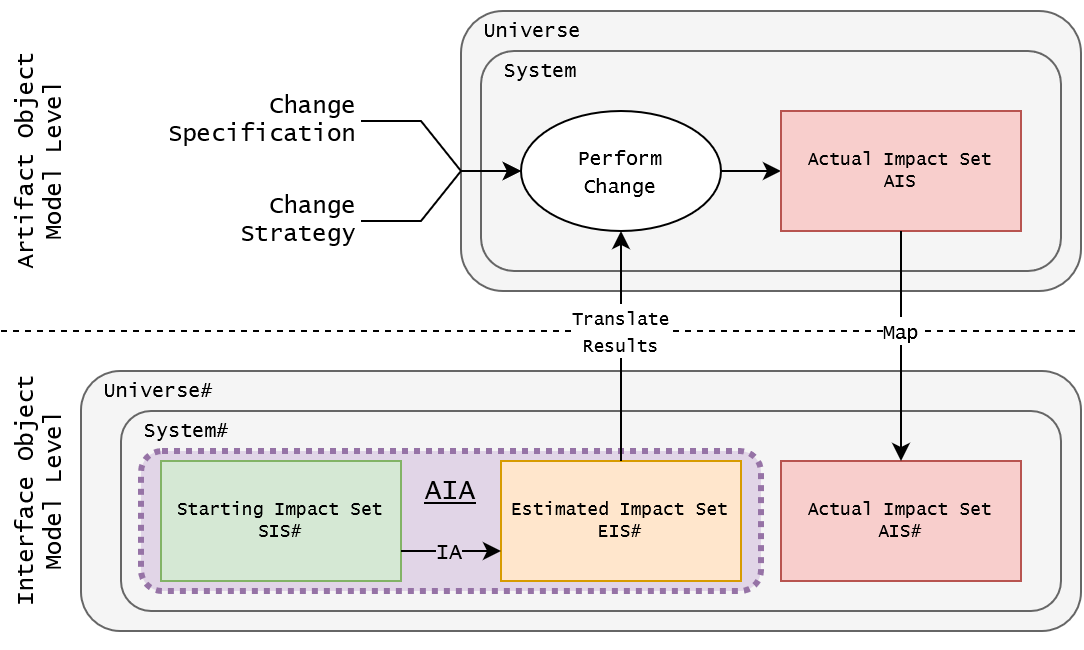
\includegraphics[width=1\linewidth]{gfx/IA35.drawio.png}
    \caption{Hauptmetriken der \ac{IA} Effektivität nach Arnold et al. \cite[296]{app_bohner}}
    [Eigene Darstellung]
    \label{fig:aia}
\end{figure}

\pagebreak

\noindent
Die definierten Mengen und Transformationen erlauben es im Folgenden Metriken zu definieren, welche Aussagen über die Genauigkeit und Effizienz des Verfahrens\footnote{der Impact-Analyse} treffen können.
Hierbei entstehen drei sinnvolle Relationen, welche man im Folgenden betrachten kann:
Die Relation zwischen der primären Anforderungsdefinition und der erarbeiteten Menge betroffener Entitäten\footnote{Bewertung der primären Änderungsdefinition}; das Verhältnis zwischen der erarbeiteten Menge betroffener Entitäten und dem Gesamtsystem\footnote{Bewertung der Eingrenzung}; und dem Abgleich der projizierten Menge betroffener Entitäten mit den eigentlich Betroffenen\footnote{Bewertung des Ergebnisses}.


\subsection{Bewertung der primären Änderungsdefinition}

Die Bewertung der primären Änderungsdefinition beschäftigt sich mit dem Verhältnis von \acsfont{SIS\#} und \acsfont{EIS\#}. 
Diese Metrik gibt Auskunft darüber, wie viele Entitäten -- die nicht durch die Änderungsdefinition vorgegeben waren -- durch die \ac{IA} als betroffen gekennzeichnet wurden.
Definitionsgemäß\footnote{nach Arnold et al.} ist es jedoch nicht möglich, dass die Analyse primär markierte Entitäten aus der Schätzung ausschließt, weshalb dessen Menge immer eine Obermenge zur Menge der primären Änderungsdefinition darstellt.

$$
    K = \dfrac{|\text{\acsfont{SIS\#}}|}{|\text{\acsfont{EIS\#}}|} \leq 1
$$

Im Rahmen der Bewertung der Impact-Analysen zu dem Thema dieser Arbeit gilt es als vorteilhaft, sowie die primäre Änderungsdefinition so genau wie möglich die Änderung des Systemes beschreibt. 

% \begin{figure}[H]
%     \centering
%     \begin{tikzpicture}
%         \begin{axis}[
%             ybar stacked,
%         	bar width=15pt,
%         	nodes near coords,
%             enlargelimits=0.15,
%             legend style={at={(0.5,-0.20)},
%               anchor=north,legend columns=-1},
%             ylabel={\#participants},
%             symbolic x coords={Erwünscht, Erwartet, Ziel},
%             xtick=data,
%             x tick label style={rotate=45,anchor=east},
%             ]
%         \addplot+[ybar] plot coordinates {(Erwünscht,1) (Erwartet,0.05) (Ziel,0.2)};
%         \addplot+[ybar] plot coordinates {(Erwünscht,0) (Erwartet,0.4) (Ziel,0.6)};
%         \addplot+[ybar] plot coordinates {(Erwünscht,0) (Erwartet,0.55) (Ziel,0.1)};
%         \legend{\strut K = 1, \strut 0.7 < K < 1, \strut K $\leq$ 0.7}
%         \end{axis}
%     \end{tikzpicture}
%     \caption{Caption}
%     \label{fig:enter-label}
% \end{figure}

\begin{table}[H]
    \centering
    \hspace*{-1.75cm}
    \begin{tabular}{rc|c|>{\centering\arraybackslash}p{0.5\linewidth}|} 
        \cline{3-4} 
        & Fallabbildung & Bedingungen & Bewertung \\\cline{3-4}
        \vspace{-1.35em} \\ \cline{3-4}
            1&\begin{minipage}{0.25\textwidth}
                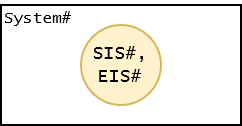
\includegraphics[width=\linewidth]{gfx/IA_1.drawio.png} 
            \end{minipage}
            &$\begin{array}{l}
                \scriptstyle EIS\# \;=\; SIS\#; \\
                \scriptstyle EIS\#,\; SIS\# \;\subseteq\; System\#
              \end{array}$ 
            &\begin{minipage}{0.5\textwidth} 
                \smaller
                \textit{Optimalfall}: Geschätzte Betroffenheit beschränkt sich auf die beschriebene Änderung.
            \end{minipage} 
            \\ \cline{3-4}
            2&\begin{minipage}{0.25\textwidth}
                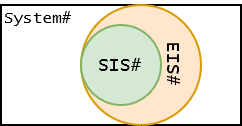
\includegraphics[width=\linewidth]{gfx/IA2.drawio.png} 
            \end{minipage}
            &$\begin{array}{l}
                \scriptstyle |EIS\#| \;>\; |SIS\#|; \\
                \scriptstyle SIS\# \;\subset\; EIS\#; \\
                \scriptstyle EIS\#,\; SIS\# \;\subseteq\; System\#
              \end{array}$ 
            & \begin{minipage}{0.5\textwidth} 
                \smaller
                \textit{Erwarteter Fall}: Die Analyse hat einige wenige Entitäten bestimmt, welche nicht in der primären Änderungsdefinition enthalten sind.
            \end{minipage} 
            \\ \cline{3-4}
            3&\begin{minipage}{0.25\textwidth}
                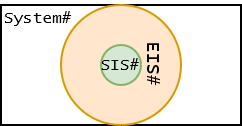
\includegraphics[width=\linewidth]{gfx/IA3.drawio.png} 
            \end{minipage}
            &$\begin{array}{l}
                \scriptstyle |EIS\#|\; \gg \; |SIS\#|; \\
                \scriptstyle SIS\# \;\subset\; EIS\#; \\
                \scriptstyle EIS\#,\; SIS\# \;\subseteq\; System\#
              \end{array}$ 
            & \begin{minipage}{0.5\textwidth}
                \smaller
                \textit{Suboptimal}: Eine große Diskrepanz zwischen \acsfont{SIS\#} und \acsfont{EIS\#} bedeutet einen höheren Arbeitsaufwand in späteren Schritten oder einer schlechten primären Änderungsdefinition.
            \end{minipage} 
            \\ \cline{3-4}
        \cline{3-4}
    \end{tabular}
    \caption{Mögliche \acsfont{SIS\#}/\acsfont{EIS\#} Abhängigkeiten nach Arnold et al. \cite[297]{app_bohner}}
    [Eigene Darstellungen]
    \label{tab:sis_eis}
\end{table}


\pagebreak

\subsection{Bewertung der Eingrenzung}

Im Weiteren kann bewertet werden, wie gut die Ergebnismenge eingeschränkt ist.
Bei der Natur einiger Änderungen kann diese Metrik auch eine Aussage darüber treffen, wie Änderungen innerhalb von Abhängigkeiten propagiert werden. 
So beschreibt ein hoher Wert der Metrik entweder ein stark vernetztes System, welches Änderungen leicht propagiert oder eine \ac{IA}, welche viele abhängige Entitäten in die Ergebnismenge mit einschließt.
Je genauer die \ac{IA} die Ergebnismenge einschränken kann, desto nützlicher ist das Ergebnis für den weiteren Prozess, da der Arbeitsaufwand so gering wie möglich bleibt. 

$$
    J = \dfrac{|\text{\acsfont{EIS\#}}|}{|\text{System\#}|} \leq 1
$$

Für die Prozesse der Nachweisführung regulativer Anforderungen ist diese Metrik direkt mit dem Arbeitsaufwand des Änderungsprozesses verknüpft.
Es gilt also im für die Bewertung einer \ac{IA} als vorteilhaft, sowie Änderungen möglichst präzise auf die betroffenen Anfoderungen eingegrenzt werden kann, da hierdurch Effizienz der Nachweisführungsprozesse verbessert werden kann.


\begin{table}[H]
    \centering
    \hspace*{-1.75cm}
    \begin{tabular}{rc|c|>{\centering\arraybackslash}p{0.5\linewidth}|} 
        \cline{3-4} 
        & Fallabbildung & Bedingungen & Bewertung \\\cline{3-4}
        \vspace{-1.35em} \\ \cline{3-4}
            1&\begin{minipage}{0.25\textwidth}
                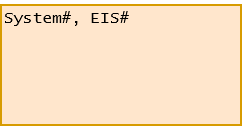
\includegraphics[width=\linewidth]{gfx/IA21.drawio.png} 
            \end{minipage}
            &$\begin{array}{l}
                \scriptstyle EIS\# \;=\; Sys\#; \\
              \end{array}$ 
            &\begin{minipage}{0.5\textwidth} 
                \smaller
                \textit{Standardfall}: Keine große Aussage für \ac{IA} kann jedoch ein System mit sehr vielen Abhängigkeiten identifizieren.
            \end{minipage} 
            \\ \cline{3-4}
            2&\begin{minipage}{0.25\textwidth}
                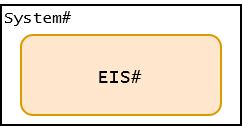
\includegraphics[width=\linewidth]{gfx/IA22.drawio.png} 
            \end{minipage}
            &$\begin{array}{l}
                \scriptstyle |System\#| \;>\; |EIS\#|; \\
                \scriptstyle EIS\# \;\subset\; System\# \\
              \end{array}$ 
            & \begin{minipage}{0.5\textwidth} 
                \smaller
                \textit{Verbesserter Fall}: Die geschätzte Änderung betrifft nicht das gesamte System und kann genauer definiert werden.
            \end{minipage} 
            \\ \cline{3-4}
            3&\begin{minipage}{0.25\textwidth}
                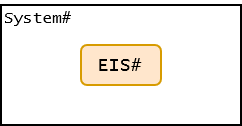
\includegraphics[width=\linewidth]{gfx/IA23.drawio.png} 
            \end{minipage}
            &$\begin{array}{l}
                \scriptstyle |System\#|\; \gg \; |EIS\#|; \\
                \scriptstyle EIS\# \;\subset\; System\# \\
              \end{array}$ 
            & \begin{minipage}{0.5\textwidth}
                \smaller
                \textit{Optimalfall}: Geschätzte Änderung beschränkt sich auf eine relativ kleine Untermenge des Systems.
            \end{minipage} 
            \\ \cline{3-4}
        \cline{3-4}
    \end{tabular}
    \caption{Mögliche \acsfont{EIS\#}/\acsfont{System\#} Abhängigkeiten nach Arnold et al. \cite[297]{app_bohner}}
    [Eigene Darstellungen]
    \label{tab:eis_sys}
\end{table}


\subsection{Bewertung des Ergebnisses}

Die letzte Metrik, welche verwendet werden kann, um die \ac{IA} zu bewerten, ist der Vergleich der ermittelten Menge mit der tatsächlich betroffenen Menge.
Die beiden Mengen\footnote{\acsfont{EIS\#} und \acsfont{AIS\#}} stellen hierbei gegenseitige keine Teil- oder Obermengen dar, weshalb die Metrik nicht begrenzt ist.
Eine zweite Metrik gibt an wie groß die Schnittmenge der beiden Mengen ist um auszuschließen, dass die Mengen keine Elemente teilen (siehe Fall 7, Tabelle \ref{tab:eis_ais}). 

$$
    H = \dfrac{|\text{\acsfont{AIS\#}}|}{|\text{\acsfont{EIS\#}}|}; \quad
    % M = \dfrac{|\text{\acsfont{EIS\#}}|}{|\text{\acsfont{AIS\#}}|}; \quad
    N = |\acsfont{AIS\#} \cap \acsfont{EIS\#}|
$$

Der Optimalfall für die Nachweisführungprozesse der Flugsicherung sollte einer der sicheren Fälle (Fälle 1-3, Tabelle \ref{tab:eis_ais}) umfassen, da diese Fälle die Vollständigkeit der Nachweisführung nicht gefährden.
Weiter beläuft sich die Differenz der Mengen im Optimalfall gegen Null, da hierdurch der manuelle Arbeitsaufwand -- Änderungen als nicht relevant zu markieren -- so gering wie möglich ausfällt.
\bigskip


\begin{table}[H]
    \centering
    \hspace*{-1.75cm}
    \begin{tabular}{rc|c|>{\centering\arraybackslash}p{0.5\linewidth}|} 
        \cline{3-4} 
        & Fallabbildung & Bedingungen & Bewertung \\\cline{3-4}
        \vspace{-1.35em} \\ \cline{3-4}
            1 & \begin{minipage}{0.25\textwidth}
                    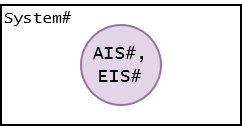
\includegraphics[width=\linewidth]{gfx/IA41.drawio.png} 
                \end{minipage}
                &$\begin{array}{l}
                    \scriptstyle EIS\# \;=\; AIS\#; \\
                    \scriptstyle EIS\# \;\subset\; System\# \\
                  \end{array}$ 
                &\begin{minipage}{0.5\textwidth} 
                    \smaller
                    \textit{Optimales Ergebnis}: Geschätzter Impact stimmt mit \acsfont{AIS\#} überein. Spricht für eine sehr hilfreiche \ac{IA}.
                \end{minipage} 
            \\ \cline{3-4}
            2 & \begin{minipage}{0.25\textwidth}
                    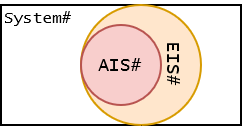
\includegraphics[width=\linewidth]{gfx/IA42.drawio.png} 
                \end{minipage}
                &$\begin{array}{l}
                    \scriptstyle |EIS\#| \;>\; |AIS\#|; \\
                    \scriptstyle AIS\# \;\subset\; EIS\#; \\
                    \scriptstyle EIS\# \;\subseteq\; System\# \\
                  \end{array}$ 
                & \begin{minipage}{0.5\textwidth} 
                    \smaller
                    \textit{Gutes sicheres Ergebnis}: Alle eingetroffenen Änderungen wurden richtig eingeschätzt und die Differenz der Mengen ist nicht sehr groß.
                \end{minipage} 
            \\ \cline{3-4}
            3 & \begin{minipage}{0.25\textwidth}
                    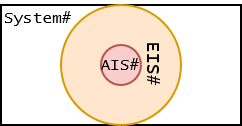
\includegraphics[width=\linewidth]{gfx/IA43.drawio.png} 
                \end{minipage}
                &$\begin{array}{l}
                    \scriptstyle |EIS\#| \;\gg\; |AIS\#|; \\
                    \scriptstyle AIS\# \;\subset\; EIS\#; \\
                    \scriptstyle EIS\# \;\subseteq\; System\# \\
                  \end{array}$ 
                & \begin{minipage}{0.5\textwidth}
                    \smaller
                    \textit{Schwaches sicheres Ergebnis}: Alle Änderungen wurden richtig eingeschätzt, jedoch ist die Differenz der Mengen sehr groß und es wurde viele weitere Entitäten falsch markiert.
                \end{minipage} 
            \\ \cline{3-4}
            4 & \begin{minipage}{0.25\textwidth}
                    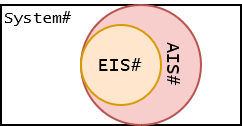
\includegraphics[width=\linewidth]{gfx/IA44.drawio.png} 
                \end{minipage}
                &$\begin{array}{l}
                    \scriptstyle |AIS\#| \;>\; |EIS\#|; \\
                    \scriptstyle EIS\# \;\subset\; AIS\#; \\
                    \scriptstyle AIS\# \;\subseteq\; System\# \\
                  \end{array}$ 
                & \begin{minipage}{0.5\textwidth}
                    \smaller
                    \textit{Unsicheres Ergebnis}: Die Abschätzung verfehlt die komplette Abdeckung aller betroffenen Änderungen.
                \end{minipage} 
            \\ \cline{3-4}
            5 & \begin{minipage}{0.25\textwidth}
                    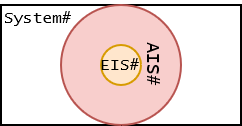
\includegraphics[width=\linewidth]{gfx/IA45.drawio.png} 
                \end{minipage}
                &$\begin{array}{l}
                    \scriptstyle |AIS\#| \;\gg\; |EIS\#|; \\
                    \scriptstyle EIS\# \;\subset\; AIS\#; \\
                    \scriptstyle AIS\# \;\subseteq\; System\# \\
                  \end{array}$ 
                & \begin{minipage}{0.5\textwidth}
                    \smaller
                    \textit{Stark unsicheres Ergebnis}: Die Abschätzung verfehlt die betroffenen Änderungen sehr. Die große Diskrepanz bedarf weiterer Arbeit zum Erschließen der \acsfont{AIS\#}.
                \end{minipage} 
            \\ \cline{3-4}
            6 & \begin{minipage}{0.25\textwidth}
                    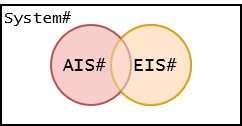
\includegraphics[width=\linewidth]{gfx/IA46.drawio.png} 
                \end{minipage}
                &$\begin{array}{l}
                    \scriptstyle |AIS\# \;\cap\; EIS\#|\; > \; 0; \\
                    \scriptstyle EIS\# \;\neq\; AIS\#; \\
                    \scriptstyle EIS\# \;\subseteq\; System\# \\
                  \end{array}$ 
                & \begin{minipage}{0.5\textwidth}
                    \smaller
                    \textit{Verfehltes Ergebnis}: Die Abschätzung verfehlt die komplette Abdeckung aller betroffenen Änderungen und beinhaltet nicht betroffene Entitäten.
                \end{minipage} 
            \\ \cline{3-4}
            7 & \begin{minipage}{0.25\textwidth}
                    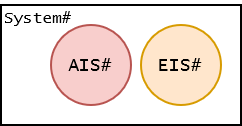
\includegraphics[width=\linewidth]{gfx/IA47.drawio.png} 
                \end{minipage}
                &$\begin{array}{l}
                    \scriptstyle |AIS\# \;\cap\; EIS\#|\; = \; 0; \\
                    \scriptstyle EIS\# \;\subset\; System\#; \\
                  \end{array}$ 
                & \begin{minipage}{0.5\textwidth}
                    \smaller
                    \textit{Stark verfehltes Ergebnis}: Extremere Version von Fall 6.
                \end{minipage} 
            \\ \cline{3-4}
        \cline{3-4}
    \end{tabular}
    \caption{Mögliche \acsfont{AIS\#}/\acsfont{EIS\#} Abhängigkeiten nach Arnold et al. \cite[299]{app_bohner}}
    [Eigene Darstellungen]
    \label{tab:eis_ais}
\end{table}


% \graffito{Dieser Teil braucht noch am ehesten Aufwand und Quellen der Rest lässt sich ziemlich runterschreiben}

% \begin{quote}
% \textcolor{red}{Einführung in den Sinn und Zweck der Impact Analyse(IA) für das erarbeitete Datenmodell und wie das Endergebnis der IA auszuschauen hat.}
% \end{quote}

